\textbf{Problem 2: Reduced-Basis Approximation.}

\begin{enumerate}[label=(\alph*),leftmargin=*,itemsep=0mm]
    
    \item Prove that in the energy norm $|||\cdot||| \equiv (a(\cdot,\cdot))^{1/2}$
    \begin{align*}
        |||u(\underline{\mu}) - u_N(\underline{\mu})||| 
        \leq |||u(\underline{\mu}) - w_N(\underline{\mu})|||,\quad\forall\>w_N\in W_N
    \end{align*}
    
    \begin{proof}
        Let $w_N(\underline{\mu}) = u_N(\underline{\mu}) + v_N(\underline{\mu})$.  Therefore, we see that
        \begin{align*}
            a(u-w_h,u-w_h) &= a((u-u_h)-v_h,(u-u_h)-v_h) \\
            &= a((u-u_h),(u-u_h)) - 2a((u-u_h),v_h) + a(v_h,v_h)
        \end{align*}
        
        By orthogonality, we have that $a((u-u_h),v_h) = 0$.  Therefore since $a(v_h,v_h)>0$ for $v_h \neq 0$, we must have that
        \begin{align*}
            |||u(\underline{\mu}) - w_N(\underline{\mu})|||^2
            = a(u-w_h,u-w_h) \geq a((u-u_h),(u-u_h))
            = |||u(\underline{\mu}) - u_N(\underline{\mu})|||^2
        \end{align*}
    \end{proof}
    
    \item Next, we wish to prove that $\underline{u}_N(\underline{\mu})$ satisfies a set of $N\times N$ linear equations
    \begin{align*}
        \underline{A}_N(\underline{\mu}) \underline{u}_N(\underline{\mu}) &= \underline{F}_N \\
        T_{\text{root}\mid N}(\underline{\mu}) &= \underline{L}_N^T \underline{u}_N(\underline{\mu})
    \end{align*}
    
    Where $\underline{A}_N(\underline{\mu}) \in \mathbb{R}^{N\times N}$, $\underline{F}_N(\underline{\mu}) \in \mathbb{R}^{N}$, $\underline{L}_N(\underline{\mu}) \in \mathbb{R}^{N}$.  Express them in terms of $\underline{A}_h(\underline{\mu}$, $\underline{F}_h(\underline{\mu}$ and $\underline{L}_h(\underline{\mu}$ respectively, and $\underline{Z}$, where $\underline{Z}$ is an $n\times N$ matrix, where the $j$-th column is $\underline{u}_h(\underline{\mu}^j)$.
    
    \begin{proof}
        
        Using the weak form $a(u_N,v) = l(v) \>\forall\>v\in w_N$, where
        \begin{gather*}
            w_N = \text{span}\> \{ u_h(\underline{\mu}^1), u_h(\underline{\mu}^1), \dots, u_h(\underline{\mu}^N) \}
        \end{gather*}
        
        Therefore, we have that
        \begin{gather*}
            v = \sum_{i=1}^N v_i u_h(\underline{\mu}^i),\quad
            u_N = \sum_{i=1}^N u_N^i u_h(\underline{\mu}^i) \\
            \therefore a \left( \sum_{i=1}^N u_N^i u_h(\underline{\mu}^i),
            \sum_{i=1}^N v_i u_h(\underline{\mu}^i) \right)
            = l\left( \sum_{i=1}^N v_i u_h(\underline{\mu}^i) \right)
        \end{gather*}
        
        From linearity and bilinearity, this simplifies to
        \begin{gather*}
            \sum_{i=1}^N \sum_{j=1}^N u_N^i v_j \cdot a(u_h(\underline{\mu}^i), u_h(\underline{\mu}^j))
            = \sum_{j=1}^N v_j \cdot l(u_h(\underline{\mu}^j))
        \end{gather*}
        
        So the problem can be written in matrix form as:
        \begin{align*}
            \underline{v}^T \underline{A}_N \underline{u}_N 
            = \underline{v}^T \underline{F}_N, \quad
            \forall\>\underline{v} \in \underline{w}_N
        \end{align*}
        
        And so we see that
        \begin{align*}
            \underline{A}_N(\underline{\mu}) \underline{u}_N(\underline{\mu}) &= \underline{F}_N
        \end{align*}
        
    \end{proof}
    
    By comparing matrix dimensions, we therefore have that
    \begin{align}
        \underline{A}_N &= \underline{Z}^T \underline{A}_h(\underline{\mu}) \underline{Z} \\
        \underline{F}_N &= \underline{Z}^T \underline{F}_h \\
        \underline{L}_N &= \underline{Z}^T \underline{L}_h
    \end{align}
    
    \item Show that the bilinear form $a(w,v;\underline{\mu})$ can be decomposed as
    \begin{align}
        a(w,v;\underline{\mu}) = \sum_{q=1}^Q \sigma^q(\underline{\mu}) a^q(w,v), \quad
        \forall\> w,v \in X, \quad \forall \>\underline{\mu} \in \mathcal{D}
    \end{align}
    
    where $Q=6$.
    
    \begin{proof}
        
        From Problem 1, part (a), we have that
        \begin{align}
            a(w,v;\underline{\mu}) &= \sum_{i=0}^4 k^i \int_{\Omega^i} \nabla u \cdot \nabla v \dd{A}
            + \int_{\Gamma\setminus\Gamma_\text{root}} \text{Bi}\cdot uv \dd{S} \nonumber\\
            &= \sum_{i=0}^4 k^i \int_{\Omega^i} \nabla u \cdot \nabla v \dd{A}
            + \text{Bi} \int_{\Gamma\setminus\Gamma_\text{root}} uv \dd{S}
        \end{align}
        
        And therefore we see that we can decompose Eq (28) into
        \begin{align}
            \underline{\sigma} &= (k^0,k^1,\dots,k^4,\text{Bi})
            = \underline{\sigma}(\underline{\mu}) \\
            a^q(w,v) &= \begin{cases}
            \int_{\Omega^q} \nabla w \cdot \nabla v \dd{A}, & \text{for $q=1,2,3,4,5$} \\
            \int_{\Gamma\setminus\Gamma_\text{root}} uv \dd{S}, & \text{for $q=6$}
            \end{cases}
        \end{align}
        
    \end{proof}
    
    And now, in that manner, we can construct an $\underline{A}_h^q$ where
    \begin{align*}
        \underline{A}_h(\underline{\mu}) = \sum_{q=1}^Q \sigma^q(\underline{\mu}) \underline{A}_h^q
    \end{align*}
    
    Comparing with Problem 1 Part (c), we have that Eq (18) is changed to
    \begin{align}
        \underline{A}_{\alpha,\beta}^{q,k} = \text{Area}^{q,k}
        (c_{x\mid\alpha}c_{x\mid\beta} + c_{y\mid\alpha}c_{y\mid\beta}) &&\quad
        1 \leq \alpha,\beta \leq 3, \quad q = 0,1,\dots,5
    \end{align}
    
    Where the area of the triangle from the local coordinates $\underline{x}^{q,k}_\beta = (x^{q,k}_\beta,y^{q,k}_\beta)$ as follows:
    \begin{align}
        \text{Area}^{q,k} = \frac{1}{2}(x_1^{q,k}(y_2^{q,k}-y_3^{q,k})
        + x_2^{q,k}(y_3^{q,k}-y_1^{q,k}) + x_3^{q,k}(y_1^{q,k}-y_2^{q,k}))
    \end{align}
    
    And for $q=6$, we have that$\underline{A}_h^{q,k}$ is given by
    \begin{align}
        \underline{A}^{q,k} &= \frac{\norm{x_2^{q,k}-x_1^{q,k}}_{L^2}}{6}
        \begin{pmatrix} 2 & 1 \\ 1 & 2 \end{pmatrix}
    \end{align}
    
    It thus follows that $\underline{A}_N(\underline{\mu}) = \underline{Z}^T \underline{A}_h(\underline{\mu}) \underline{Z}$ can be broken down into
    \begin{align}
        \underline{A}_N(\underline{\mu}) &= \sum_{q=1}^Q \underline{Z}^T \underline{\sigma}^q \underline{A}_h^q(\underline{\mu}) \underline{Z}
        = \sum_{q=1}^Q \underline{\sigma}^q \underline{A}_N^q(\underline{\mu}) \\
        \text{where}\> \underline{A}_N^q(\underline{\mu})
        &= \underline{Z}^T \underline{A}_h^q(\underline{\mu}) \underline{Z}
    \end{align}
    
    \item I coded up offline/online version of the reduced-basis approximation following the computational decomposition indicated below.  Based on the data that we were given \texttt{sn.dat} and $\mu_0$, we verified that the $T_{\text{root}\mid N}(\underline{\mu}_0) = 1.72621$, and for the $\underline{\mu}_1 = \{1.8,4.2,5.7,2.9,0.3\}$ combination, we calculate $T_{\text{root}\mid N}(\underline{\mu}_1) = 1.07485$.
    
    \item Using the Newton's optimization method, we consider a thermal fin with specified thermal conductivities $\{k_1,k_2,k_3,k_4\} = \{0.4,0.6,0.8,1.2\}$, and the Biot number over ranges $\text{Bi} = [0.1,10]$.  We also determine the cost function as
    \begin{align}
        C(\text{Bi}) = 0.2\>\text{Bi} + T_\text{root}(\text{Bi})
    \end{align}
    
    From our results, we see that $C$ is minimized at $\text{Bi} = 1.32966$, corresponding to a cost function of $C=0.92551$ and a temperature of $T_\text{root}=0.65958$ (Fig. \ref{prj2_qn2_pte}).

    \begin{figure*}[h!]
    \centering
    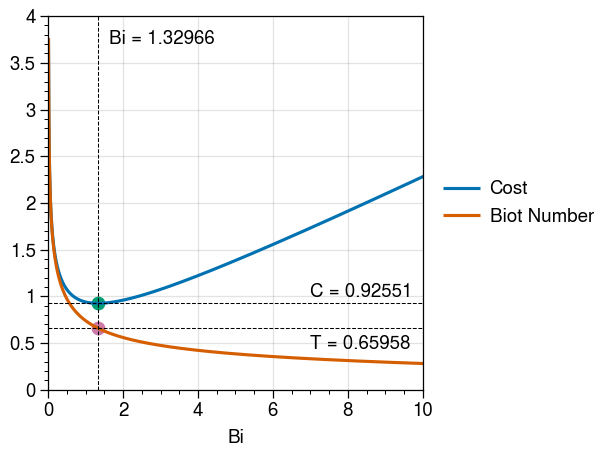
\includegraphics[width=0.6\textwidth]{figures/prj2_qn2_pte.png}\\
    \caption{}
    \label{prj2_qn2_pte}
    \end{figure*}
    
\end{enumerate}